\documentclass[a4paper,12pt,titlepage]{article}
\usepackage[T1]{fontenc}
\usepackage[brazil]{babel}
\usepackage[utf8x]{inputenc}
\usepackage{graphicx}
\usepackage{times}
\usepackage{ucs}
\usepackage{url}




\title{Relatório final: \\Bolsa PIBIC \\CNPQ} 


\author{Aluno: Rodrigo L. M. Flores \and
        Orientador: Roberto Hirata Jr. }


\date{\today}

\begin{document}

\maketitle

\nocite{wiki:volunteercomputing}
\nocite{wiki:interpretedlanguage}
\nocite{wiki:boinc}
\nocite{wiki:r}
\nocite{boinc_wrapper}
\nocite{hungaro}
\nocite{nytimes}

\part{Parte objetiva}

\section{Introdução}

O ponto de partida para este projeto vem da necessidade de se fazer processamentos custosos de 
dados em bioinformática. Estes processamentos costumam ser combinatórios, o que os fazem
demorar um bom tempo sendo executados em um computador comum, sendo necessário utilizar recursos
computacionais de alta performance para obter os resultados em tempo hábil.

\subsection{Programação paralela e distribuída}

Uma abordagem clássica para se resolver esse problema é utilizar \textit{clusters} que são um grupo de computadores
ligados entre si de modo a parecer ser um único computador muito mais potente. \textit{Clusters} podem ser tanto máquinas
específicas para isso, produzidas com um alto custo e com um hardware específico para otimizar seu desempenho, ou 
pode ser utilizado o conceito de computação em grades: utilizar computadores comuns trabalhando em paralelo 
para fazer o processamento. 

Uma outra alternativa é utilizar grades computacionais distribuídas. Grades computacionais costumam ser constituídas
de um conjunto de computadores cujo principal objetivo não é fazer processamento pesado, mas sim lidar com o usuário 
cotidiano que normalmente utiliza a máquina para acessar a internet, ler seu correio eletrônico, elaborar
trabalhos usando processadores de texto e planilhas eletrônicas, entre outras coisas. Embora grades computacionais tenham um 
processamento menor que clusters dedicados, costumam ter um custo muito menor, já que normalmente computadores ``comuns'' já existem em
uma empresa ou universidade. 


\subsection{Computação voluntária}
%Bibliografia Wikipedia


A computação voluntária é um tipo de computação distribuída no qual pessoas que possuem computadores podem doar processamento e
armazenamento ocioso de suas máquinas enquanto elas estiverem ociosas. Estes projetos normalmente têm um objetivo bem definide.

O primeiro projeto de Computação voluntária foi o \textit{Great Internet Mersenne Prime Search}, lançado em janeiro de 1996. 
Seu objetivo era encontrar números primos de Mersenne\footnote{Isto é, números primos na forma $M_n = 2^n - 1$}. Em seguida houveram 
muitos outros projetos e alguns utilizam um apelo social, de modo a obter mais doadores de processamento, um exemplo disso é o
o Folding At Home, que investiga o enrolamento de proteínas e que pode ajudar o desenvolvimentos de pesquisas contra 
Câncer, doença de Huntington, entre outras. 

Um dos projetos mais notáveis de computação voluntária foi o \textit{SETI@Home}. Os objetivos iniciais deste projeto eram: 

\begin{itemize}
  \item Provar a viabilidade e a praticidade de grades computacionais distribuídas;
  \item Fazer um trabalho útil e apoiar uma análise de observações para detectar vida inteligente fora da Terra.
\end{itemize}

Este projeto atraiu centenas de milhares de voluntários, porém só o primeiro objetivo teve sucesso: não foram encontrados sinais 
de vida inteligente fora da Terra. Um middleware então foi criado para este fim: o \textit{BOINC}. 

\subsection{Linguagens Interpretadas}

%Colocar bibliografia da wikipedia

Uma das possíveis divisões para linguagens de programação é se seus códigos são compilados ou simplismente interpretados. Enquanto no primeiro caso
é necessária a utilização de um programa para transformar o código fonte em código de máquina para ele poder então ser executado. No segundo caso,
há a figura de um interpretador que não converte o programa para código de máquina, mas sim o interpreta e o executa. 

Linguagens interpretadas possuem vantagens e desvantagens: embora elas sejam mais fáceis de serem multiplataforma (basta o interpretador
estar disponível para aquela plataforma)e permitam escopo e tipagem dinâmica, também costumam ser menos eficientes que linguagens compiladas e 
a presença de um interpretador é obrigatória para sua execução. 

Dentre as linguagens interpretadas, uma que adquiriu destaque na área de estatística e bioinformática é a linguagem \emph{R}, que também 
pode ser utilizado como um ambiente. Esta linguagem já vem com as distribuições estatísticas mais usuais e possui uma extensibilidade 
forte com bibliotecas que podem ser baixadas facilmente.


\subsection{Linguagens interpretadas e computação distribuída}

Embora já existam ótimas soluções para a execução distribuída de programas compilados como o
 MPI\footnote{disponível em \url{http://www.mcs.anl.gov/research/projects/mpi/}}, não se fala muito em soluções 
para execução distribuída de programas em linguagem interpretada. 
Para a linguagem \emph{R} há um pacote chamado \emph{gridR} que permite o uso do R com o \emph{Condor}, %Colocar note
um middleware para execução de programas em grades.  Um outro trabalho que relaciona o R com computação distribuída é o %Colocar o artigo do Rodrigo


O artigo %Colocar bibliografia
sobre a utilização do Middleware de computação voluntária BOINC como solução para computação 
em grade na Universidade de Extremadura na Espanha. Dentre os programas executados na grade, haviam
programas em R. Porém isso foi somente instalado em redes de computadores com computadores cujo sistema
operacional é o Linux. 

Seguindo este feito, este trabalho tem a intenção de construir algo semelhante nos laboratórios da rede CEC do IME/USP. Utilizando
não somente os computadores executando Linux, mas também os computadores cujo sistema operacional é o Microsoft Windows %Colocar marca registrada.
já que estes são uma parte considerável da rede.  



\newpage

\section{Conceitos e tecnologias utilizadas}

O desenvolvimento do projeto incluiu diversas tecnologias, sendo as principais a linguagem de Programação \emph{R} e o middleware
para computação voluntária \emph{Boinc}. Dentre os conceitos estudados, podemos destacar a computação em grade.  

\subsection{BOINC}

O BOINC, cujo nome é uma sigla para \textit{Berkeley Open Infrastructure for Network Computing}, é um middleware 
para computação em grade e voluntária e foi criado na Universidade de Berkeley, Califórnia, Estados Unidos.

Inicialmente, o projeto consistia em gerenciar o projeto \textit{SETI@HOME} que possuía dois objetivos:

\begin{itemize}
	\item Provar a viabilidade e a praticidade do conceito ``computação em grade distribuída'';
	\item Fazer um trabalho científico útil fazendo uma análise observacional para detectar vida inteligente fora da Terra.
\end{itemize}

O primeiro objetivo foi concluído com sucesso e o resultado é o \textit{BOINC}. O segundo falhou: nenhuma evidência de 
vida inteligente fora da Terra foi encontrada. 

Dentre os diversos motivos para a utilização do \emph{BOINC}, baseados no artigo \cite{boinc}, podemos destacar:

\begin{itemize}
  \item \textbf{Mais utilizado -} Quando comparado com outros \emph{middlewares} semelhantes como o \textit{middleware} 
\emph{Condor} ou o \emph{Xtremweb}, o \emph{BOINC} é mais utilizado e há pacotes para o \emph{BOINC} nas 
distribuições \emph{Linux} mais populares;
  \item \textbf{Amplamente utilizado -} O \emph{BOINC} é utilizado em diversas áreas como previsão do tempo, física
astrofísica, biologia, entre outras;
  \item \textbf{Suporte da comunidade -} Baseado no espírito de ajuda mútua existente em comunidades de software livre, é 
possível ter dúvidas esclarecidas quanto ao funcionamento do \emph{BOINC} de maneira fácil e desburocratizada. Por ser um projeto
cujas listas de discussão e canais de \textit{chat} são movimentados é bem comum alguns problemas serem resolvidos em questão de 
poucos dias;
  \item \textbf{Estrutura simples -} O BOINC possui uma estrutura simples de comunicação: um servidor que armazena e 
distribui os trabalhos a serem feitos e os clientes que tem o papel de processar os trabalhos;
  \item \textbf{Documentação completa -} A página oficial do BOINC possui muita documentação e muitos tutoriais explicando
cada detalhe da instalação e configuração de um projeto. Há também páginas não oficiais como o %Wiki não oficial do BOINC
que também servem de ajuda.
\end{itemize}



\subsubsection{Funcionamento do BOINC}


Cada unidade de processamento no Boinc é chamada de \emph{workunit} e é constítuida de arquivos executáveis e 
arquivos de entrada. Depois de processado, os arquivos de saída gerados são enviados para o servidor que
normalmente armazena estes arquivos em um banco de dados ou em um arquivo.

Para gerar um workunit são necessários dois arquivos XML, um deles detalhando a entrada e o 
outro detalhando a saída. Para facilitar a escrita do programa, precisamos escrever para cada arquivo um nome lógico 
que ao enviar e receber o cliente renomeia o arquivo. Por exemplo, temos um programa que lê um arquivo chamado 
\verb#input# e escreve no arquivo \verb#output#, para podermos ter muitos arquivos de entrada com nomes diferentes, quando
criamos uma \emph{workunit}, o servidor coloca um nome único e semelhante ao da workunit nos arquivos de entrada e saída que serão renomeados
pelo cliente para o nome lógico.

O processamento é realizado pelo cliente: o arquivo binário é executado e enquanto ele é executado há um checkpoint
que permite em caso de interrupções retomar o processamento de um determinado ponto. Finalizado o processamento, 
na próxima atualização o cliente avisará ao servidor que o processamento foi finalizado. Um diagrama do funcionamento pode
ser visto na figura \ref{funcionamento-boinc}. 


\begin{figure}[!h]
  \centering
  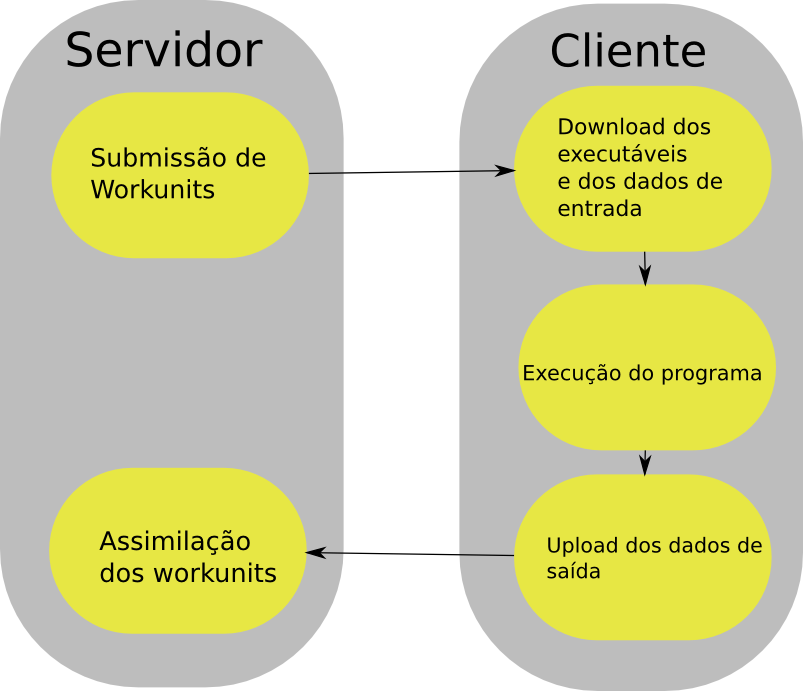
\includegraphics[scale=0.5]{boinc-schema.png}
  \caption{Funcionamento do Boinc}
  \label{funcionamento-boinc}
\end{figure}

\newpage

\subsubsection{Wrapper}


O \emph{Wrapper} é um programa escrito utilizando a \emph{api} do \emph{BOINC}, cujo objetivo é executar aplicações legadas, 
i.e. aplicações que não utilizam a API do \emph{BOINC}, utilizando o \textit{BOINC}. Há uma versão do Wrapper distribuída junto com o 
\textit{BOINC} que utiliza um arquivo XML, mas existe uma outra opção descrita no artigo \cite{hungaro} que utiliza um shell para a 
execução dos aplicativos. Os diagramas de funcionamento do 
\emph{BOINC} com um programa escrito com a api e com o wrapper podem ser vistas nas figuras \ref{boinc-api} e \ref{boinc-wrap} 
respectivamente.


O arquivo XML de execução tem a seguinte estrutura:

\begin{verbatim}
<job_desc>
    <task>
        <application>foobar</application>
        [ <stdin_filename>stdin_file</stdin_filename> ]
        [ <stdout_filename>stdout_file</stdout_filename> ]
        [ <stderr_filename>stderr_file</stderr_filename> ]
        [ <command_line>--foo bar</command_line> ]
    </task>
    [ ... ]
</job_desc>
\end{verbatim}

Neste XML, o único campo obrigatório é o \emph{application}, que é a aplicação
que será executada e pode ser distribuída junto com a aplicação ou já existir no 
computador que o cliente estará instalado (para este segundo caso é necessário
informar o caminho inteiro do executável). É possível ter mais de uma tag
task, e o wrapper as executará sequencialmente. É de responsabilidade
do \textit{Wrapper} perceber se a execução do programa foi feita com sucesso, 
mas não é responsabilidade dele verificar se os pré-requisitos que o programa necessida
estão presentes no sistema. 


\begin{figure}[!h]
  \centering
  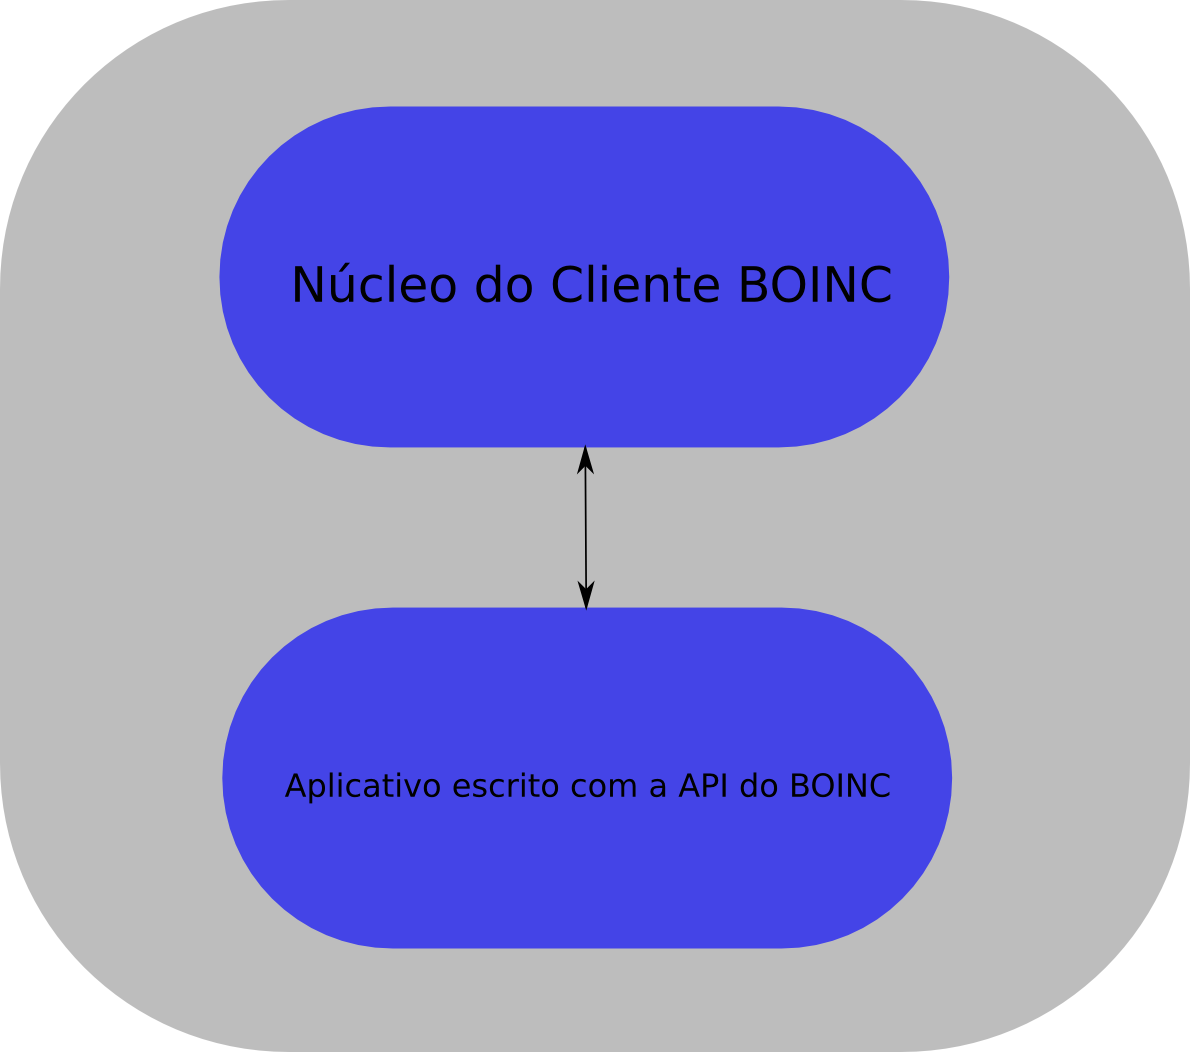
\includegraphics[scale=0.3]{boinc-api.png}
  \caption{Funcionamento do Boinc utilizando uma aplicação que utiliza sua api}
  \label{boinc-api}
\end{figure}


\begin{figure}[!h]
  \centering
  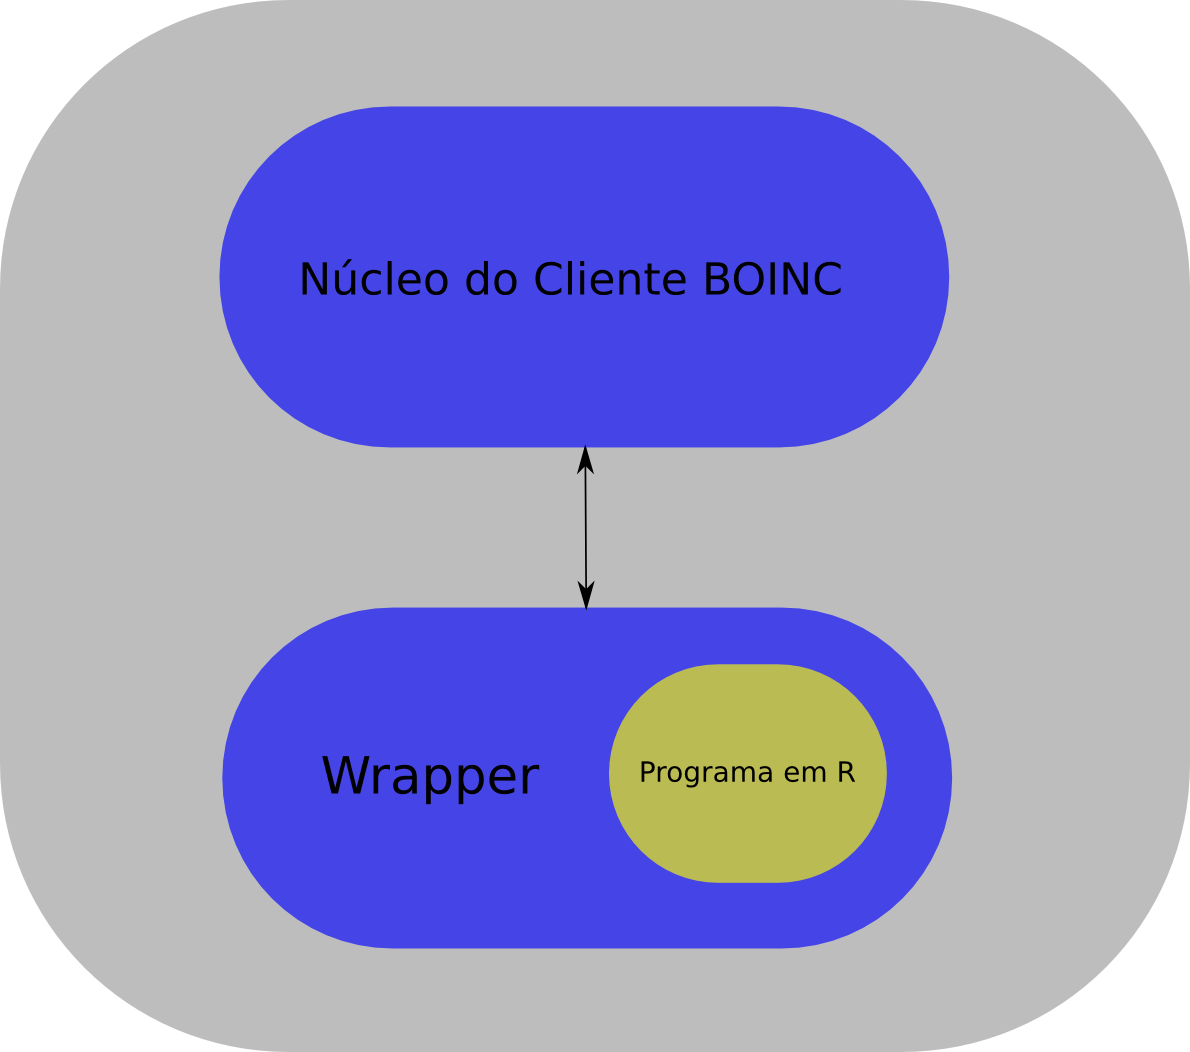
\includegraphics[scale=0.3]{boinc-wrap.png}
  \caption{Funcionamento do Boinc utilizando uma aplicação que utiliza o \emph{wrapper}}
  \label{boinc-wrap}
\end{figure}


\subsection{R}

A linguagem de programação estatística \emph{R} é uma implementação da linguagem \emph{S} e foi criada por Ross Ihaka e Robert
Gentleman na Universidade de Auckland, da Nova Zelândia. A linguagem e ambiente para cálculos estatísticos é considerada
padrão %http://www.nytimes.com/2009/01/07/technology/business-computing/07program.html?_r=1
na área de análise de dados e além do ambiente acadêmico, empresas como \emph{Google}, \emph{Pfizer} e \emph{Merck} a utilizam em seus
processos de mineração de dados. 

Dentre as facilidades que seu uso proporciona, podemos citar as seguintes:

\begin{itemize}
  \item Grande quantidade de funções estatísticas de uso cotidiano na análise de dados
como cálculo de média, desvio padrão, ajuste de curvas, análise de séries temporais. Há também funções mais complexas como por 
exemplo implementações de algoritmos de \emph{clustering}. 
  \item Utilizando o \emph{R} é possível fazer operações em tabelas semelhantes a que normalmente 
são feitas em bancos de dados relacionais como seleção de linhas em tabelas que atendem
certas condições. 
  \item O \emph{R} possui também rotinas de manipulação de matrizes e resolução de sistemas lineares, que são essenciais
em qualquer tarefa de cálculo numérico. 
  \item Gráficos de alta qualidade dos mais variados tipos e para os mais variados propósitos com uma qualidade alta 
também podem ser feitos com o \emph{R}. 
  \item A facilidade de se criar e de se obter pacotes, que nada mais são que conjuntos de rotinas agrupadas, é outro fator
importante: é muito simples criar pacotes e documentá-los. Para disponibilizá-los, pode se submeter um pedido de aprovação 
de para disponibilização no repositório oficial (\url{http://cran-r.c3sl.ufpr.br/})  
do \emph{R}, que possui $2076$ pacotes para os mais diversos fins. O repositório possui \emph{mirrors} espalhados por
todo o mundo, inclusive no Brasil.  
\end{itemize}

Além destes motivos, o artigo \cite{bioconductor} dispõe outros motivos para a utilização do \emph{R} e de seu
pacote para análise de dados de de bioinformática \emph{Bioconductor}.

\begin{itemize}
  \item \textbf{Transparência -} Muitas metodologias de análise na área de biologia e bioinformática computacional
são extremamente complexas e muitas etapas são necessárias na conversão de informação bruta (como por exemplo imagens 
escaneadas de \emph{microarray}). Não se sabe a priori, como as análises podem ser sensíveis a estes fatores, e portanto
trabalhos referenciados na área normalmente expõe todo o processo. O uso de mesmo ambiente e das mesmas facilita bastante
esta transparência;
  \item \textbf{Reprodutibilidade -} Experimentos na área de biologia molecular devem publicar listas de ingredientes
e algoritmos para criar substâncias e processos. Um resultado só pode ser verificado se existir uma obediência a 
um protocolo. Seguindo esta linha, a mineração de dados também deve ser bem descrita e tanto o código fonte 
como os dados nos quais a análise é baseada são normalmente publicados junto com um trabalho nesta área. Utilizar
um mesmo ambiente, que pode ser obtido gratuitamente, para as qualquer plataforma, com pacotes 
facilmente extensíveis também facilita este processo.
  \item \textbf{Eficiência do desenvolvimento -} Se pacote foi por ventura desenvolvido para alguma necessidade, ele pode ser publicado
, melhorado, estudado por outros cientistas, e pode ter seu leque de funcionalidades aumentado caso seu uso siga padrões
de código aberto. Para isso é necessário que esteja bem documentado. Tanto o \emph{R} como o \emph{Bioconductor} são softwares
de código aberto e disfrutam desta qualidade.
  \item \textbf{Prototipagem -} Como o \emph{R} é uma linguagem em um nível mais alto que outras linguagens como \emph{C} ou
\emph{FORTRAN}, programar novas rotinas é bem mais simples. Mesmo não tendo uma execução tão eficiente como em outras
linguagens, pode ser utilizado como protótipo, para depois ser implementado em uma linguagem mais eficiente caso o 
resultado seja bom. 

\end{itemize}

\subsection{Utilização \emph{BOINC} para o processamento de rotinas na linguagem \emph{R}}

Dentre as possibilidades de processamento em grade para a linguagem \emph{R}, escolhemos o \emph{BOINC} para o processamento em grade.
Dentre os motivos, podemos citar:

\begin{itemize}
  \item \textbf{Código aberto -} Ambas as tecnologias são de código aberto e possuem licenças que permitem a utilização das duas
ferramentas para qualquer propósito, além da obtenção gratuita e d possibilidade de estudo do código fonte das duas tecnologias.
Outro ponto forte em comum entre elas é a presença de uma comunidade ativa, com fóruns, listas de discussão e canais de IRC;
  \item \textbf{Multiplataforma -}  Em redes de universidades e empresas é muito comum a utilização de sistemas tanto 
\emph{Linux} como \emph{Windows}. Em ambientes nos quais há muito desenvolvimento de programas, o \emph{Linux} acaba
sendo bastante utilizado, já para um usuário cotidiano o Windows acaba sendo o sistema utilizado. Ter uma solução
que utilize tanto computadores com sistemas \emph{Linux} como computadores com sistemas \emph{Windows} é essencial 
para sua utilização. Como o \emph{R} e o \emph{BOINC} já tem versões para estes dois sistemas, assim como o \emph{wrapper}, 
fica então possível a utilização multiplataforma da grade. Lembrando que a utilização multiplataforma deve funcionar para um mesmo
projeto e sem distinção de workunits, de modo a ser indiferente à quem submete a utilização de qual sistema para a computação.
  \item \textbf{Execução inalterada de aplicações escritas em \emph{R} -} Utilizando o \emph{wrapper} é possível executar,
sem precisar alterar um byte do código, programas compilados. Utilizando como programa compilado o interpretador do 
\emph{R}, podemos executar rotinas do \emph{R} em utilizando o \emph{wrapper}. Isso poupa o trabalho de reescrever
códigos já previamente escritos e em funcionamento;
  \item \textbf{Possibilidade de se utilizar pacotes do \emph{R} -} Como o \emph{R} possui uma notável extensibilidade com mais
de $2000$ pacotes, é de se esperar que um ambiente para executar rotinas nesta linguagem também seja capaz de automaticamente instalar
pacotes do \emph{R}, caso isto seja necessário. Utilizando o \emph{BOINC} e o \emph{wrapper} é possível utilizar estes pacotes,
sendo apenas necessário verificar se eles estão instalados e colocar no programa o comando de instalação caso não estejam.
\end{itemize}


\newpage

\section{Atividades realizadas}


O início do projeto deu-se ainda em 2008, com a visita ao colégio Rainha da Paz na Lapa, onde o aluno de mestrado do \textit{IME}
Rodrigo Assirati Dias mantém uma grade de computadores com o middleware \textit{Alchemi} citada no trabalho \cite{Dias}
. Nesta visita foi possível esclarecer dúvidas, entender o funcionamento da grade e receber algumas dicas quanto à manutenção da grade. 
Após esse encontro, começou-se a buscar alternativas para o a computação de alta performance com o \textit{R}. Um primeiro pacote encontrado
que fazia esta função foi o \textit{GridR}, que permite submeter rotinas do \textit{R} para \textit{clusters}, máquinas remotas e 
grades. Um dos arcabouços possíveis para o uso deste pacote é o Condor\footnote{Disponível em \url{http://www.cs.wisc.edu/condor/}}
, desenvolvido pela \textit{University of Wisconsin-Madison} e é bastante utilizado em empresas
de grande porte como a \textit{NASA} e pode ser executado tanto em sistemas
baseados em \textit{UNIX}, como em sistemas \textit{Windows}. Seguindo esta busca, encontramos o 
\textit{middleware} \textit{BOINC}, no artigo \cite{boinc}
sendo utilizado para um propósito semelhante em um trabalho na Universidade de Extremadura, na Espanha 
e decidimos que a abordagem seria interessante para nosso trabalho.

Escolhido o \textit{middleware} nos focamos na instalação do servidor. A própria página do \textit{BOINC} 
possui um guia de instalação do servidor do \textit{middleware} no sistema \textit{Debian GNU\Linux} e por
esta distribuição \textit{Linux} ser bastante conhecida por sua estabilidade, foi instalado este sistema no servidor.
Instalado o servidor, o foco foi em ter uma aplicação em R executando remotamente em uma grade de computadores. 
Este processo no sistema Linux foi relativamente simples: utilizando o ``truque do \textit{shebang}'' é possível 
colocar um script como executável e o \textit{wrapper} executá-lo como se fosse um arquivo compilado. Já para
o sistema Windows %Colocar marca registrada
o trabalho foi mais complicado: havia um bug nas configurações de compilação do \textit{wrapper} e até perceber isso
atrasou bastante o andamento do projeto. Passado isso, foi necessário utilizar um programa escrito em C, que apenas executava 
o interpretador junto com o arquivo com a rotina em \textit{R}.

Finalizado esta parte, nos focamos na aplicação a ser executada na grade. Para isso foi criado um programa em \textit{R} que
apenas acessava um arquivo e fazia alguns cálculos custosos. Isto foi então configurado para o mesmo programa poder
ser executado tanto em sistemas Windows como em sistemas Linux. Paralelamente a isso, foi pedido para a administração
da rede do \textit{CEC} para instalar o \textit{BOINC} nas máquinas da rede. Como a rede estava em reforma, para a troca
do sistema operacional não foi possível concluir a instalação até o fim deste trabalho, mas acredito que em breve teremos a grade em 
pleno funcionamento.




\newpage

\section{Resultados e produtos obtidos}


O principal resultado deste trabalho foi fazer o \emph{Boinc} funcionar com rotinas em \emph{R}, tanto
nos ambientes \emph{Linux} como no ambiente \emph{Windows} % colocar marca registrada

\subsection{Implementação}

\subsubsection{Sistema Linux}

Para o ambiente \emph{Linux}, foi relativamente simples o processo: dado um arquivo com rotinas
do \emph{R} a serem executadas, é somente necessário alterar a permissão do arquivo para executável 
(via \verb#chmod +x arquivo.R#) e adicionar a seguinte linha no início do arquivo:

\begin{verbatim}
#!/usr/bin/Rscript
\end{verbatim}

Isso faz um sistema \emph{Linux} chamar o interpretador \emph{Rscript} para interpretar o arquivo  
e assim fazer a interpretação do arquivo. Esta solução permite não só que rotinas em \emph{R} sejam
executadas, mas sim qualquer script que tenha seu interpretador descrito na primeira linha.

A esta solução, demos o nome de \emph{Truque do Shebang}, pelos caracteres \verb'#!' serem chamados
popularmente de \emph{shebang}. Esta implementação foi relativamente simples: o BOINC possuía um tutorial
para executarmos programas compilados na grade e só o truque do shebang foi necessário.

Porém, para termos a mesma solução em ambos os sistemas, utilizamos a solução para
Windows no sistema Linux. 

\subsubsection{Sistema Windows} %Marca registrada

Como o sistema Windows não permite utilizar script utilizando o \emph{shebang}, foi necessário 
utilizar um programa compilado escrito na linguagem C, que chamamos de \emph{Runner}, 
que usando a função \verb#system#, chama o interpretador com o arquivo.R como parâmetro. 

Esta solução permite inclusive que usemos scripts diferentes de R a cada vez que criamos um 
\emph{workunit}, assim como adicionar arquivos extra que por ventura fossem necessários para
o processamento. Esta maneira também funciona no \emph{Linux}, só que o \emph{Runner} precisar
ser compilado para o \emph{Linux} com o caminho para o interpretador correto. O programa também não faz
uma verificação para perceber se o \emph{R} está instalado. 

A utilização do \emph{Runner} foi necessário devido ao \emph{Wrapper} não perceber corretamente
que o interpretador foi executado sem erros e mesmo em execuções sem erros, o \emph{wrapper} 
recebia um valor de retorno do interpretador diferente de zero, o que ele percebia como um erro
e marcava o \emph{workunit} como inválido. Um diagrama exemplificando esse funcionamento pode ser visto 
na figura \ref{diagrama-boinc-wrapper-windows}. Para a execução ficar multiplataforma, foi necessário 
fazer uma pequena alteração no \emph{wrapper} na versão para \emph{Linux} modificando o nome do
arquivo XML do wrapper, já que em ambos os sistemas é necessária a utilização de um arquivo XML próprio.


A implementação no Windows foi bastante difícil: existem muitos pequenos detalhes que acabam
atrapalhando um pouco. Um dos exemplos foi especificar o caminho do executável: para o Windows acessar
um diretório específico devemos ``truncar'' os nomes de diretórios maiores que $8$ caracteres, sendo 
assim o diretório trocando o oitavo e nono caractere por \verb#~1# e desprezando os seguintes. 
Alguns outros problemas foram relacionados à falta de mensagens de erro do BOINC mais amigáveis e
à falta de verificação das entradas: um \verb#XML# mal formatado causou um erro  no processamento
do workunit, quando isso deveria ser acusado na submissão do workunit. Outro problema foi um \emph{Bug}
nas configurações de compilação do \emph{wrapper} no Microsoft Visual Studio Express % Verificar 
que fazia referência a bibliotecas desnecessárias e inexistentes para a compilação do \emph{wrapper}
e isso só foi resolvido pelos desenvolvedores do \emph{BOINC} algumas semanas depois. 


\begin{figure}[!h]
  \centering
  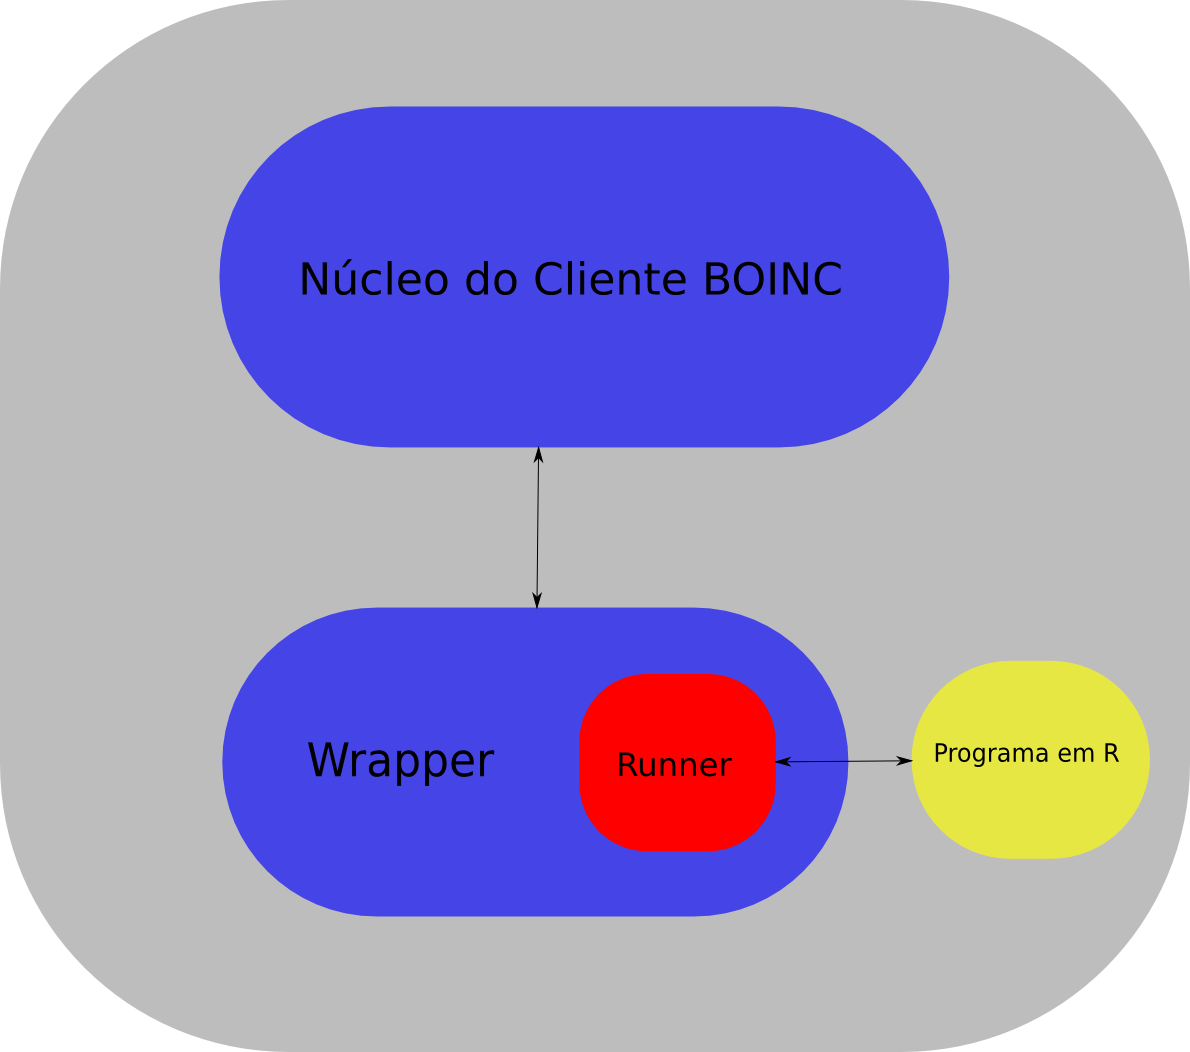
\includegraphics[scale=0.3]{boinc-diagram-runner.png}
  \caption{Diagrama do funcionamento do \emph{BOINC} com o \emph{Runner} e \emph{Wrapper}}
  \label{diagrama-boinc-wrapper-windows}
\end{figure}
 

\subsection{Discussão}



\subsubsection{Vantagens} 

As principais vantagens no uso do \emph{Boinc} para o processamento em grade são:

\begin{itemize}
  \item \textbf{Facilidade de se adicionar novos nós} - A instalação do BOINC em ambos os sistemas Linux e Windows é simples
e fácil de ser feita e nenhuma ação no servidor é necessária a cada instalação de nós. Além disso, é muito simples fazer
a replicação de configurações, tanto para o processamento, quanto para a conexão com o servidor para os computadores;
  \item \textbf{Processamento multiplataforma} - Para a grade funcionar na plataforma só são necessárias duas coisas: 
que o BOINC e o \emph{R} estejam disponível para a plataforma. As plataformas mais comuns 
(Linux $32$ e $64$ bits e Microsoft Windows) têm ambos os projetos disponíveis;
  \item \textbf{Código aberto} - A utilização de dois softwares com código aberto facilita bastante: a 
busca de bugs se torna possível, a gratuidade dos softwares e a grande quantidade de documentação, muitas vezes produzidas por
pessoas que não necessariamente são da equipe de desenvolvimento do \emph{BOINC}. A mentalidade de ajuda mútua, existente nas
listas de discussão e no canal de IRC do projeto também é de grande ajuda; 
  \item \textbf{Execução invisível ao usuário} - Com o \emph{BOINC} configurado para isso, um usuário comum da rede nem ao menos 
percebe a existência de um processamento em grade. É possível configurar o \emph{BOINC} para só começar a execução com o computador ocioso
após um número arbitrário de minutos. Também é possível configurar para o processamento só acontecer em determinadas 
faixas de horários e dias da semana. Outra configuração interessante é a determinação do máximo de memória 
\emph{RAM} e de espaço em disco para a execução, assim como a frequência com que ele usará a rede. 
  \item \textbf{Solução funciona para qualquer linguagem de script} - De maneira análoga, é possível executar qualquer programa escrito em 
linguagem interpretada com o BOINC utilizando esta mesma solução. Como comentado antes, só é necessário que exista uma versão do interpretador
para as plataformas necessárias (o que é comum para as linguagens mais utilizadas como \emph{PERL}, \emph{Python} e 
\emph{Ruby} e as plataformas mais comuns). 

\end{itemize}

\subsubsection{Desvantagens}

As principais desvantagens são:

\begin{itemize}
  \item \textbf{Necessidade de se ter o \emph{R} instalado} - O \emph{R} não é uma linguagem instalada por padrão
nas distribuições Linux mais populares, nem no \emph{Windows}. Então, a adição de um nó só pode ser feita se o \emph{R}
for também instalado. 
  \item \textbf{Falta de checkpoints} - Utilizando um aplicativo feito com a \emph{API} do \emph{BOINC} é possível se ter
\emph{Checkpoints}, que são uma maneira de uma aplicação feita com o \emph{BOINC} reiniciar o processamento
não do início, mas sim de um determinado ponto. Utilizando o \emph{Wrapper} e o \emph{R}, perdemos esse recurso. A computação
de rotinas longas se torna mais difícil e pouco recomendada, já que a cada interrupção o processamento é reiniciado. 
  \item \textbf{Falta de ``compromisso'' fixo dos clientes} - Diferentemente da rede citada no artigo \cite{Dias}
não há a figura de um computador \emph{Manager} que gerencia as máquinas, atualizando a qualquer momento, mas sim um servidor 
que apenas envia e recebe as tarefas e a iniciativa de computação fica com os computadores da grade. 

\end{itemize}

\subsection{Instalação da rede}

A instalação está em andamento na rede do laboratório CEC do IME-USP. No momento possuímos $3$ máquinas Linux e $2$ máquinas Windows com o \emph{Boinc}
em funcionamento . Por motivos de reinstalação do sistema dos computadores, a instalação está tomando 
mais tempo que o previsto, mas em breve acredito que teremos a grade em seu pleno funcionamento.




\newpage

\section{Conclusões}


A principal conclusão deste trabalho é que é possível a utilização do \emph{BOINC} para o processamento
de rotinas de bioinformática escritas na linguagem \emph{R}. A utilização multiplataforma
também foi de grande utilidade já que podemos incluir praticamente qualquer tipo de computador 
existente em redes. O custo total de implementação foi somente a inutilização de uma máquina, utilizada
como servidor da rede. Embora o \emph{BOINC} seja um projeto consolidado e possua uma documentação com bastante conteúdo,
as mensagens de erro, principalmente do \emph{Wrapper}, são muito pouco informativas, o que tornou o desenvolvimento 
deste projeto bastante trabalhoso. 

Para a continuação do projeto há várias sugestões:

\begin{itemize}
  \item \emph{Benchmark} da rede e comparação com grade descrita no artigo \cite{Dias}
Para determinar a viabilidade, seria interessante estabelecermos a comparação com outra 
alternativa. 
  \item Comparação com grades ``alugadas'': hoje já existe oportunidade de se fazer esse tipo de processamento.
em grades alugadas como a oferecida pela empresa \emph{Amazon}. Como os computadores na rede 
consomem energia elétrica seria interessante comparar o gasto da energia elétrica com o gasto em 
uma grade ``alugada''.
  \item Analisar o desempenho nas máquinas com Windows e com Linux. Seria interessante analisar 
o Benchmark da grade em ambos os sistemas e determinar qual das duas plataformas é mais
propícia para o processamento;
  \item Utilização de máquinas virtuais: como feito no artigo \cite{boinc}, podemos utilizar
máquinas virtuais, que são iniciadas em cada nó e é feito o processamento. Sem ter que se preocupar
com a instalação do \emph{R} em todas as máquinas 
\end{itemize}




\newpage

\bibliographystyle{amsalpha}
\bibliography{bibliografia}


\newpage


\part{Parte subjetiva}

% desafios e frustrações encontrados;
% lista das disciplinas cursadas no BCC mais relevantes para o trabalho;
% observações sobre a aplicação de conceitos estudados nas disciplinas do curso;
% se o aluno fosse continuar atuando na área em que realizou o trabalho, que passos tomaria para aprimorar os conhecimentos relevantes para esta atividade?

\section{Desafios e frustrações encontrados}

O curso de bacharelado em ciência da computação é um curso bastante denso e dificilmente temos tempo
para fazer todas as tarefas de todas as disciplinas. Então acredito que o meu maior desafio nestes anos de IME 
foi conciliar todas as tarefas e disciplinas, e infelizmente descartando alguma as vezes. 

A falta de aprendizado de orientação a objeto também foi uma frustração: como este assunto é muito requisitado por empresas
e projetos, não aprendê-lo foi bastante frustrante. Há também pouco enfoque a tecnologias, deveriam haver mais chances de
aprendermos tecnologias e desenvolvermos mais projetos. 

Para algumas disciplinas também que pedem projetos e trabalhos únicos que são entregues no decorrer do semestre, 
falta uma coisa muito importante: um \emph{Feedback} constante do professor/monitor para saber se estamos no caminho certo. 
No decorrer do curso conclui algumas matérias com trabalhos que eu acreditei estar bom, mas com uma nota abaixo do esperado. 
Fazer um trabalho de conclusão de curso também é uma escolha muito feliz: serve para coroarmos nosso aprendizado
e aplicá-los utilizando os temas que mais gostamos.  

A figura de um orientador e de um tutor também foi de suma importância: é sempre interessante ter alguém que se possa receber
conselhos de matérias e de optativas. Desenvolver também um projeto de iniciação científica também foi importante, para 
meu desenvolvimento e acredito que para qualquer aluno seria uma experiência válida. 

 

\section{Disciplinas relevantes para o trabalho}

Diversas disciplinas foram relevantes para este trabalho:

\begin{itemize}
  \item \textbf{MAC122 - Principio e desenvolvimento de algoritmos } - Este curso fornece uma base importante para as outras matérias e
ajuda a melhorar o raciocínio para elaborarmos algoritmos.
  \item \textbf{MAC323 - Estruturas de Dados } - Aprender as diversas estruturas de dados, seu uso e a eficiência é essencial
para qualquer trabalho que envolva ciência da computação.
  \item \textbf{MAC211 - Laboratório de programação I} - Ferramentas como versionamento de código, processamento de 
texto e o makefile foram essenciais para a elaboração deste trabalho de forma indireta e contribuíram com a 
boa qualidade do mesmo.
  \item \textbf{MAC242 - Laboratório de programação II} - Linguagens de script facilitam bastante o trabalho de tarefas 
repetitivas e o boa parte do que sei sobre este tipo de linguagem eu aprendi neste curso.
  \item \textbf{MAC338 - Análise de algoritmos} - Este curso contribuiu indiretamente com minha formação como cientista da computação i
e muitos dos conceitos aprendidos neste curso ajudaram o entendimento melhor de algoritmos e soluções.
  \item \textbf{MAC431 - Programação paralela e distribuída} Aprender a utilidade de programação de alta performance foi de bastante utilidade
neste trabalho.
  \item \textbf{MAC422 - Sistemas Operacionais} - Saber como um programa é executado, como o sistema gerencia essas execução e como a tabela de processos
funciona é essencial quando se trabalha com uma grade de computadores. 
  \item \textbf{IBI5031 - Reconhecimento de padrões} - Neste curso tive a oportunidade de aprender algoritmos e fazer análises de dados, 
que são normalmente feitas em pesquisas de bioinformática. Também programei bastante na linguagem \emph{R} neste curso e percebi sua
importância
\end{itemize}

\section{Conceitos Aplicados}

Dentre os conceitos aprendidos no curso utilizados no trabalho pode-se citar a computação distribuída, aprendida no curso de
computação paralela e distribuída. Saber que alguns problemas só podem ser resolvidos de uma exaustiva, também 
foi importante e esse foi um conceito aprendido no curso de Análise de Algoritmos.  


\section{Continuação do trabalho}

O trabalho possui uma continuação óbvia: terminar a instalação em todos os nós da rede e fazer uma análise de \emph{Benchmarking da rede} para
testar a viabilidade quando a instalação estiver completa, como resultado disso há a possibilidade de
escrevermos um artigo falando sobre a grade para ser publicado na página do \emph{BOINC}. Outro trabalho interessante decorrente deste 
seria melhorar o \emph{Wrapper} e o \emph{BOINC} em geral para fazê-los terem mensagens de erros mais claras. 

\section{Agradecimentos}

Este trabalho foi feito com a ajuda de diversas pessoas. Indiretamente, meus pais, familiares, amigos e namorada foram de extrema importância 
no apoio, amizade e carinho. 

Diretamente, agradeço à CNPq pela bolsa que me permitiu a dedicação exclusiva a este projeto. Agradeço também ao meu orientador, 
Prof. Dr. Roberto Hirata Jr. que me apoiou e me ajudou bastante na elaboração deste trabalho. Para a obtenção do servidor,
agradeço ao Prof. Dr. Roberto Marcondes César Junior, e aos administradores da Rede Vision, David Pires e Rodrigo Bernardo Pimentel, 
que me ajudaram quando na substituição do servidor com um problema de \emph{hardware}. Agradeço também ao aluno de pós-graduação
Rodrigo Assirati Dias, que me ajudou e me deu diversas dicas com relação à manutenção e a instalação da grade. Na parte do \emph{BOINC}
agradeço à Nicolás Alvarez e Yoyo, que me ajudaram a resolver os bugs e a implementar a solução descrita pelo trabalho. Agradeço também 
o Prof. Dr. Alfredo Goldman pela disponibilização da rede \emph{CEC} e aos administradores da rede, Jânio Matsuura e Gislaine Olivi
pela instalação da grade.






\end{document}
